\subsubsection{Unstructured meshes}\label{unstructured-meshes}

\noindent Unstructured meshes can be abstractly viewed as a collection of sets 
(e.g. nodes, edges, cells, etc.), data defined on these sets (e.g. fluxes, 
coordinates, velocities), and explicit connectivity information between 
sets. The connectivity information, declared as mapping tables are required for 
determining the neighbors of a set element. If we represent sets as consecutive 
indices from zero to the size of the set, then the mapping between two 
sets is represented as an array which stores the index of set elements in the 
second set of the mapping (referred to as the to-set) for every set element of 
the first set (known as the from-set). For the majority of such applications, 
the number of to-set elements connected to each from-set element is fixed (e.g. 
all edges have two vertices). For example consider the mesh illustrated 
in Figure~\ref{fig:unstructured}. Part of the mappings from edges to cells for 
this mesh is detailed in Figure~\ref{fig:mapping}. Given such a mapping, we can 
access the index of those elements that are connected to the current element of 
the from-set from other sets (the to-sets of the mappings). 

The computations on the mesh are declared as a loop over the elements of a set, 
executing some block of computation on each set element (i.e. an elemental kernel), 
while accessing data directly on the iteration set or indirectly through a 
mapping.  If a loop over a set only writes to data defined on that set during the 
elemental kernel, then each iteration of the loop could run in parallel. 
However, for kernels that indirectly increment data, there may be multiple 
from-set iterations that update the same to-set element. Such indirect-loops are 
common in finite volume and finite element applications over 
unstructured-meshes: e.g. when updating state variables in cells using fluxes 
across faces, or when doing matrix assembly. The parallelization of indirect 
loops are non-trivial as the exact elements leading to data races cannot be 
determined from compile time information, given that they are driven by the 
structure of the mesh in general and the mapping tables in particular, which are 
read in during run-time. 

% The sole focus of the research is this paper is this indirect-loop data access 
% pattern. 


\begin{figure}
\centering

\includegraphics[width=4cm]{fig/svg/unstructured.eps}
\caption{Unstructured mesh, the arrow represents the mapping tells $e_i$ is
  connected to $c_j$ and $c_k$.}
\label{fig:unstructured}
\end{figure}



\begin{figure}
\centering
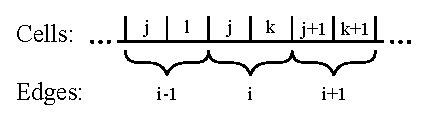
\includegraphics[width=6cm]{fig/svg/mapping.eps}
\caption{A part of the mapping from edges to cells.}
\label{fig:mapping}
\end{figure}


Some restrictions that apply is also worth noting here. The first is the use of 
only a single level of mappings. This means that every piece of data that is 
accessed during an iteration over a set is either defined directly on that set, 
or is accessed through at most one level of indirection. However, this 
restriction does not exclude applications using nested indirections, since a 
mapping table can be created to contain the indexes that we access through 
multiple mappings. The second restriction is that the result of the operations 
on the sets are independent from the order of processing the elements of the 
sets (within machine precision). This restriction enables to exploit the 
maximum opportunities for parallelization given that the accuracy of the 
algorithms do not depend on the order of execution. Finally, only  mappings with 
a fixed number of connections (or arity) are considered; such as edges to 
vertices (where the degree is always 2), unlike for a vertices to vertices 
mapping, where this will vary. The natural formalization of most FEM and FV 
algorithm uses mappings with fixed number of connections.

In spite of the above restrictions, the contributions of the research detailed 
in this paper is sufficiently general to be applicable to applications that has 
a computational steps described as an iteration on a set, accessing data on the 
set and indirectly via a mapping (with a fixed arity). Examples include 
assembly, certain types of linear algebra algorithms, flux computations, etc.
